%%%%%%%%%%%%%%%%%%%%%%%%%%%%%%%%%%%%%%%%%%%%%%%%%%%%%%%%%%%%%%%%%%%%%%%%%%%%
%%%%%%%%%%%%%%%%%%%%%%%%%%%%%%%%%%%%%%%%%%%%%%%%%%%%%%%%%%%%%%%%%%%%%%%%%%%%

\documentclass[letterpaper,twocolumn,10pt]{article}

\setlength{\textheight}{9.0in}
\setlength{\columnsep}{0.25in}
\setlength{\textwidth}{6.50in}

\setlength{\topmargin}{0.0in}
\LARGE
\setlength{\headheight}{0.0in}
\setlength{\headsep}{0.0in}
%\usepackage{times}
\usepackage{stfloats}
\usepackage{wrapfig}
\usepackage{amsmath}
\usepackage{amssymb}
\usepackage{enumerate}
\usepackage{tikz}
\usepackage{amsthm}
\usepackage{balance}
\usepackage{url}
\usepackage{relsize}
\usepackage{comment}
\usepackage{multirow}
\usepackage{booktabs}
\usepackage{array}
\usepackage{footmisc}
\usepackage{xspace}
\usepackage{pslatex}
\usepackage{microtype}
\usepackage{graphicx}
\usepackage{listings}
\usepackage{fmtcount}

\usepackage{paralist}
\usepackage[tight]{subfigure}
\usepackage[compact]{titlesec}
\usepackage{hyperref} % include this last

\theoremstyle{plain}
\newtheorem{theorem}{\bf{Theorem}}%[section]
\newtheorem{procedure}{\bf{Procedure}}%[section]
\newtheorem{lemma}[theorem]{\bf{Lemma}}
\newtheorem{corollary}[theorem]{\bf{Corollary}}
\newtheorem{proofl}[theorem]{\bf{Proof}}

\theoremstyle{definition}
\newtheorem{definition}{\bf{Definition}}%[section]
\newtheorem{observation}{\bf{Observation}}%[section] 
\theoremstyle{remark}
\newtheorem{example}{\bf{Example}}
\newtheorem{notation}{\bf{Notation}}
\newtheorem{fact}{\bf{Fact}}

% To avoid bad hypens:
\hyphenation{InvariMint}

\newcommand{\MC}{\mathbb{C}}
\newcommand{\MCI}{\mathbb{C}_{\infty}}
\newcommand{\MR}{\mathbb{R}}
\newcommand{\MZ}{\mathbb{Z}}
\newcommand{\MN}{\mathbb{N}}
\newcommand{\MS}{\mathbb{S}}

\newcommand{\AP}{\leftarrow}
\newcommand{\AFby}{\rightarrow}
\newcommand{\NFby}{\not\rightarrow}

%% Bring items closer together in list environments
%% This doesn't work with an optional argument to the list environment.
% Prevent infinite loops
\let\Itemize =\itemize    
\let\Enumerate =\enumerate
\let\Description =\description
% Zero the vertical spacing parameters
\def\Nospacing{\itemsep=0pt\topsep=0pt\partopsep=0pt\parskip=0pt\parsep=0pt}
% Redefine the environments in terms of the original values
\renewenvironment{itemize}{\Itemize\Nospacing}{\endlist}
\renewenvironment{enumerate}{\Enumerate\Nospacing}{\endlist}
\renewenvironment{description}{\Description\Nospacing}{\endlist}


% \|name| or \mathid{name} denotes identifiers and slots in formulas
\def\|#1|{\mathid{#1}}
\newcommand{\mathid}[1]{\ensuremath{\mathit{#1}}}
% \<name> or \codeid{name} denotes computer code identifiers
\def\<#1>{\codeid{#1}}
\newcommand{\codeid}[1]{\ifmmode{\mbox{\ttfamily{#1}}}\else{\ttfamily #1}\fi}

% At least 80% of every float page must be taken up by
% floats; there will be no page with more than 20% white space.
\def\topfraction{.8}
\def\dbltopfraction{\topfraction}
\def\floatpagefraction{\topfraction}     % default .5
\def\dblfloatpagefraction{\topfraction}  % default .5
\def\textfraction{.2}

% Add line between figure and text
\makeatletter
\def\topfigrule{\kern3\p@ \hrule \kern -3.4\p@} % the \hrule is .4pt high
\def\botfigrule{\kern-3\p@ \hrule \kern 2.6\p@} % the \hrule is .4pt high
\def\dblfigrule{\kern3\p@ \hrule \kern -3.4\p@} % the \hrule is .4pt high
\makeatother
% Reduce space between figures and text
\addtolength{\textfloatsep}{-.5\textfloatsep}
\addtolength{\dbltextfloatsep}{-.5\dbltextfloatsep}
% Optional
\addtolength{\floatsep}{-.5\floatsep}
\addtolength{\dblfloatsep}{-.5\dblfloatsep}




%%%%%%%%%%%%%%%%%%%%%%%%%%%%%%%%%%%%%%%%%%%%%%%%%%%%%%%%%%%%%%%%%%%%%%%%%%%%
% Formatting
%%%%%%%%%%%%%%%%%%%%%%%%%%%%%%%%%%%%%%%%%%%%%%%%%%%%%%%%%%%%%%%%%%%%%%%%%%%% 

\intextsep 5pt plus 2pt minus 4pt      % Space between in-text figures and
%%                                         % text.

\textfloatsep 5pt plus 2pt minus 4pt   % Space between main text and floats
%%                                         % at top or bottom of page.


\dbltextfloatsep 5pt plus 2pt minus 4pt   % Space between main text and floats
%%                                         % at top or bottom of page.

\setlength{\abovecaptionskip}{1pt}
\setlength{\belowcaptionskip}{1pt}

%\def\ffsp{\def\baselinestretch{0.99}\large\normalsize}

\let\oldthebibliography=\thebibliography
\let\endoldthebibliography=\endthebibliography
\renewenvironment{thebibliography}[1]{%
\begin{oldthebibliography}{#1}%
\setlength{\itemsep}{-.3ex}%
}%
{%
\end{oldthebibliography}%
}

\def\topfraction{.9}
\def\textfraction{.1}

%%%%%%%%%%%%%%%%%%%%%%%%%%%%%%%%%%%%%%%%%%%%%%%%%%%%%%%%%%%%%%%%%%%%%%%%%%%%
% Macros
%%%%%%%%%%%%%%%%%%%%%%%%%%%%%%%%%%%%%%%%%%%%%%%%%%%%%%%%%%%%%%%%%%%%%%%%%%%% 

% Switches for determining document version

\newcommand{\eat}[1]{}

% Different font in captions
\newcommand{\captionfonts}{\small}

\makeatletter
\long\def\@makecaption#1#2{%
  \vskip\abovecaptionskip
  \sbox\@tempboxa{{\captionfonts #1: #2}}%
  \ifdim \wd\@tempboxa >\hsize
    {\captionfonts #1: #2\par}
  \else
    \hbox to\hsize{\hfil\box\@tempboxa\hfil}%
  \fi
  \vskip\belowcaptionskip}
\makeatother

\newcommand{\smallcaption}[1]{%
\vspace{-2mm}%
\begin{small}\caption{#1}\end{small}%
\vspace{-2.5mm}
}

\newcommand{\todo}[1]{\textbf{\textcolor{red}{[TODO: #1]}}}

\newcommand{\etal}{et al.}
\newcommand{\parahead}[1]{\textbf{\textit{#1}}}
\newcommand{\heading}[1]{{\vspace{6pt}\noindent\bf{#1}\hspace{6pt}}}

%%%%%%%%%%%%%%%%%%%%%%%%%%%%%%%%%%%%%%%%%%%%%%%%%%%%%%%%%%%%%%%%%%%%%%%%%%%%
% Package configuration
%%%%%%%%%%%%%%%%%%%%%%%%%%%%%%%%%%%%%%%%%%%%%%%%%%%%%%%%%%%%%%%%%%%%%%%%%%%%

\theoremstyle{definition}
\newtheorem{condition}{Condition}[section]

\lstdefinelanguage{cs}
{
  morekeywords={abstract,event,new,struct,as,explicit,null,switch
        base,extern,this,bool,false,operator,throw,
        break,finally,out,true,byte,fixed,override,try,
        case,float,params,typeof,catch,for,private,uint,
        char,foreach,protected,ulong,checked,goto,public,unchecked,
        class,if,readonly,unsafe,const,implicit,ref,ushort,
        continue,in,return,using,decimal,int,sbyte,virtual,
        default,interface,sealed,volatile,delegate,internal,short,void,
        do,is,sizeof,while,double,lock,stackalloc,
        else,long,static,enum,namespace,string,
        where, from, select, group,by, having, into, many,
        last, every,
        or, and, on, var, when,let, zip, combine,
        minute,hour,day,week,year,calendar,count, Delay, Until, TakeUntil, Sample, Skip, Throttle},
      sensitive=true,
      morecomment=[l]{//},
      morecomment=[s]{/*}{*/},
      morestring=[b]",
}

\lstset{
    language=cs,
    tabsize=2,
        basicstyle=\footnotesize,
        %upquote=true,
%        aboveskip={1.5\baselineskip},
        columns=fullflexible, %fixed,
        showstringspaces=false,
        extendedchars=true,
        breaklines=true,
%      prebreak = \raisebox{0ex}[0ex][0ex]{\ensuremath{\hookleftarrow}},
%   frame=single,
        showtabs=false,
        showspaces=false,
       identifierstyle=\ttfamily,
        keywordstyle=\color[rgb]{0,0,1},% \sffamily,
        commentstyle=\color[rgb]{0.133,0.545,0.133},
%        stringstyle=\color[rgb]{0.627,0.126,0.941},
    numbers=left,
    xleftmargin=17pt,
%   tabsize=2
    captionpos=b,
    breakatwhitespace=true,     % sets if automatic breaks should only happen at whitespace
}

\hypersetup{
   pdftitle = {InvariMint: Modeling Logged Behavior with Invariant DFAs},
   pdfauthor = {Jenny Abrahamson},
   bookmarks=true,         % show bookmarks bar?
   unicode=false,          % non-Latin characters in AcrobatÕs bookmarks
   pdftoolbar=true,        % show AcrobatÕs toolbar?
   pdfmenubar=true,        % show AcrobatÕs menu?
   pdffitwindow=false,     % window fit to page when opened
   pdfstartview={FitH},    % fits the width of the page to the window
   pdfnewwindow=true,      % links in new window
   colorlinks=true,        % false: boxed links; true: colored links
   linkcolor=black,          % color of internal links
   citecolor=black,        % color of links to bibliography
   filecolor=black,      % color of file links
   urlcolor=black           % color of external links
}

%%%%%%%%%%%%%%%%%%%%%%%%%%%%%%%%%%%%%%%%%%%%%%%%%%%%%%%%%%%%%%%%%%%%%%%%%%%% 
% Metadata
%%%%%%%%%%%%%%%%%%%%%%%%%%%%%%%%%%%%%%%%%%%%%%%%%%%%%%%%%%%%%%%%%%%%%%%%%%%%

%\date{\today} % no date

%\conferenceinfo{SLAML 2011,} {October 23, 2011, Cascais, Portugal.} 
%\CopyrightYear{2011} 
%\crdata{978-1-4503-0443-6/11/09} 
%\clubpenalty=10000 
%\widowpenalty = 10000

\title{InvariMint: Modeling Logged Behavior with Invariant DFAs}

% 11 point font
\newcommand{\headerfont}[1]{{\fontsize{12pt}{13.6pt}\selectfont #1}}

\author{
\headerfont{Jenny Abrahamson}\\\\
\headerfont{Computer Science \& Engineering}\\
\headerfont{University of Washington}
}

%%%%%%%%%%%%%%%%%%%%%%%%%%%%%%%%%%%%%%%%%%%%%%%%%%%%%%%%%%%%%%%%%%%%%%%%%%%% 
% Front Matter
%%%%%%%%%%%%%%%%%%%%%%%%%%%%%%%%%%%%%%%%%%%%%%%%%%%%%%%%%%%%%%%%%%%%%%%%%%%%

\begin{document}

\maketitle

% Turn off page numbers
%\pagestyle{empty}
\thispagestyle{empty}


%%%%%%%%%%%%%%%%%%%%%%%%%%%%%%%%%%%%%%%%%%%%%%%%%%%%%%%%%%%%%%%%%%%%%%%%%%%%
% Content
%%%%%%%%%%%%%%%%%%%%%%%%%%%%%%%%%%%%%%%%%%%%%%%%%%%%%%%%%%%%%%%%%%%%%%%%%%%%

%%%%%%%%%%%%%%%%%%%%%%%%%%%%%%%%%%%%%%%%%%%%%%%%%%%%%%%%%%
\subsection*{Abstract}
%%%%%%%%%%%%%%%%%%%%%%%%%%%%%%%%%%%%%%%%%%%%%%%%%%%%%%%%%%
We present a semantic parsing approach for temporal expression resolution. 
Previous work, including current state of the art approaches, primarily use pattern matching and regular expression-like rules for grounding temporal expressions. However, the compositionality of language suggests a more linguistically principled approach. 

In our system, using a hand-built lexicon and CCG parser, we first construct a 
base CCG parse for each temporal phrase, then build a set of candidate
context-dependent logical forms from each base parse. We learn to select one parse from this set using a perceptron and features based on the logic, the phrase itself, and, critically, the full context the in which the phrase appears. Finally, we execute this logical form to a standardized date and time representation. This approach builds on previous successes using CCG for semantic parsing, and using a small featureset of linguistically motivated features, we achieve moderate accuracy on task A of TempEval3.

%%%%%%%%%%%%%%%%%%%%%%%%%%%%%%%%%%%%%%%%%%%%%%%%%%%%%%%%%%
\section{Introduction}
\label{sec:introduction}
%%%%%%%%%%%%%%%%%%%%%%%%%%%%%%%%%%%%%%%%%%%%%%%%%%%%%%%%%%

% 1. Problem my system is trying to solve:
Temporal expression resolution is the task of mapping from a 
Temporal phrases are ubiquitous. They appear in all kinds of text, from e-mail to newswire to Wikipedia articles. 
Much of the information in print and Internet media consists of text that describes events occurring at a specific point in time. For a computer to be able to comprehend this text, it will need to be able to recognize events, and reason about how they are located temporally. Building a system that can understand temporal relations in text is a first step toward a system that can understand much of the information available in news articles, scientific journals and on the Internet.
Improved reasoning about times and events will enable us to build more effective systems for question answering, information extraction, and summarization. For example, a system that had extracted the two relations CEO(Steve Jobs, Apple) and CEO(Tim Cook, Apple) wouldn’t be able to answer the question “Who is the CEO of Apple?” It would also need to understand the temporal relationship between the two relations.


%Figure~\ref{fig:motivating-log} presents a log snippet from a hypothetical


% Roadmap of what's up next
In section 2 we cover previous work on this problem. Then, in section 3, we go over our representation and approach to parsing. Section 4 reveals our learning. Section 5 shows our results. Finally, section 6 talks about future work.



%%%%%%%%%%%%%%%%%%%%%%%%%%%%%%%%%%%%%%%%%%%%%%%%%%%%%%%%%%
\section{Motivation}
\label{sec:motivation}
%%%%%%%%%%%%%%%%%%%%%%%%%%%%%%%%%%%%%%%%%%%%%%%%%%%%%%%%%%
\begin{figure}
   {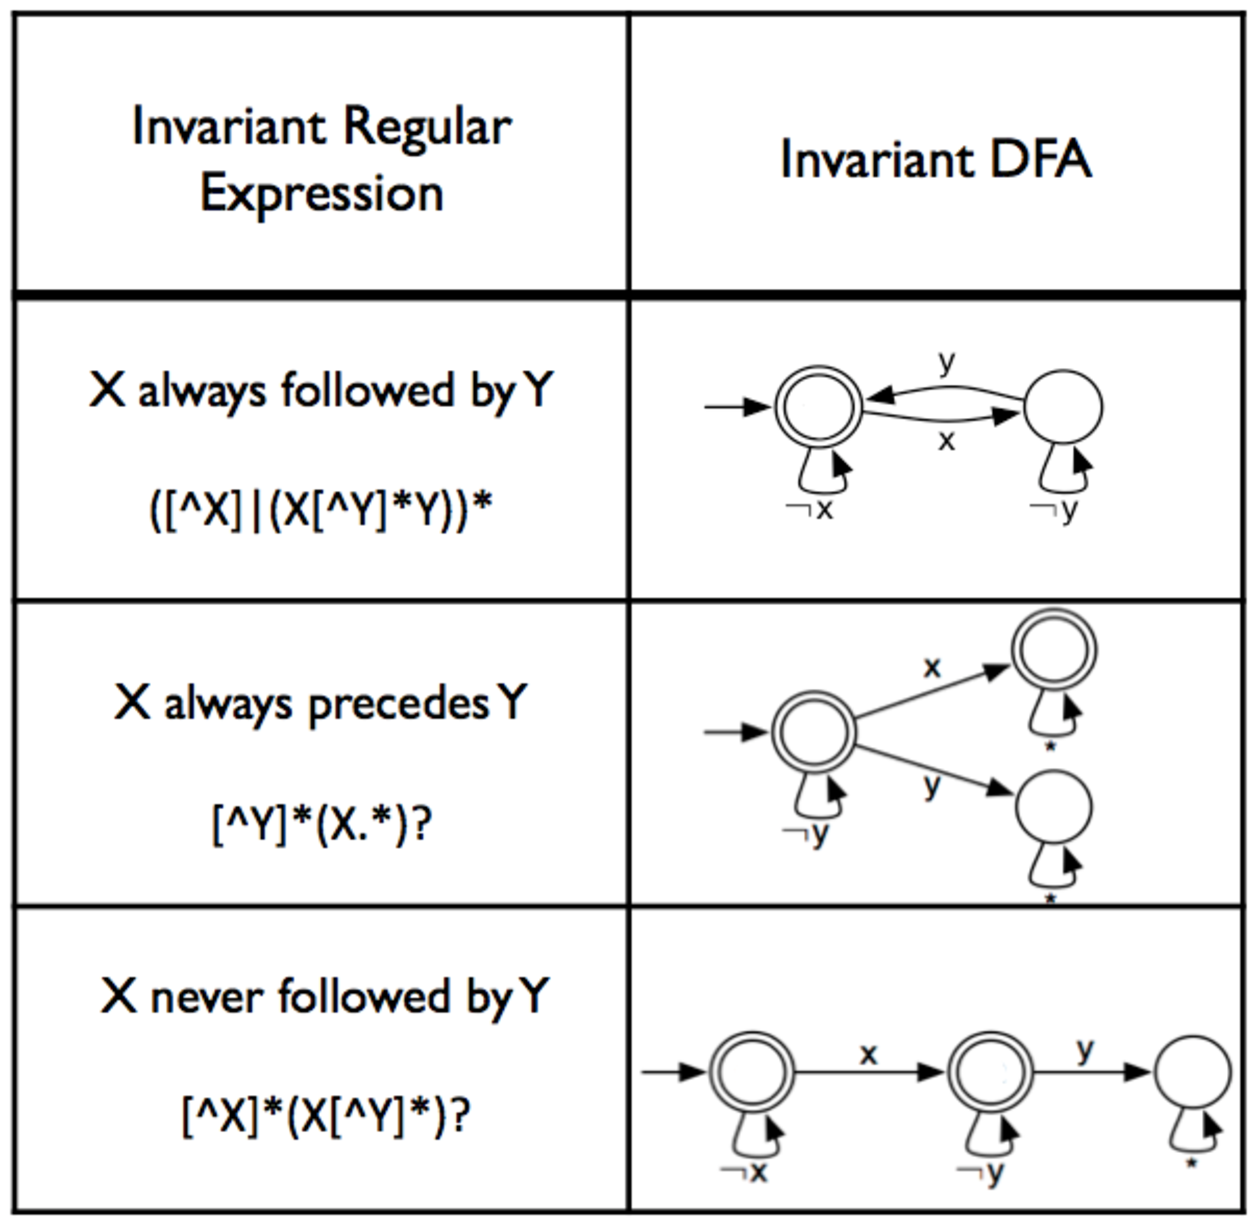
\includegraphics[width=\columnwidth]{fig/invRegexDfa.pdf}}
   \caption{The regular expressions used to translate each invariant type into
   an
   invariant DFA.
    } 
   \label{fig:invRegDfa}
\end{figure}
In addition to efficiency, the formal languages perspective is poised to improve
upon a number of other Synoptic shortcomings. 

First, Synoptic itself is not very flexible.
Built into many places of its implementation are assumptions about the three explicitly
mined invariants described in Section~\ref{sec:synoptic}. Adding a new invariant would require new invariant
miner, model checker, and counter-example generator code. So while it is
certainly possible to incorporate new invariants, there are a large
number of potentially useful invariants and each individually would require 
substantial effort to implement. 

Second, though intended for developers, Synoptic is challenging for users to
understand as the aggregate process is complex. For the final model to be most
helpful, we believe that users would benefit from understanding the process
that generated the model.

Finally, there is not a known optimal way to choose the order in which
invariants are satisfied during Synoptic's refinement phase. This problem
introduces nondeterminism into the process, as the order in which invariants are
satisfied affects the final model and can cause non-optimal refinement
steps. Synoptic is thus not guaranteed to find a globally minimal 
model satisfying all invariants, and will generate an arbitrary locally minimal
model. Because smaller models are easier to analyze,
the global minimum is preferred. 

As we will soon see, InvariMint addresses each of these deficiencies. But first, a
more formal treatment of its approach.

%%%%%%%%%%%%%%%%%%%%%%%%%%%%%%%%%%%%%%%%%%%%%%%%%%%%%%%%%%
\section{Formalizing the technique}
\label{sec:formalizing}
%%%%%%%%%%%%%%%%%%%%%%%%%%%%%%%%%%%%%%%%%%%%%%%%%%%%%%%%%%

This section defines the formalisms used by InvariMint, explains the process
used to construct a model equivalent to Synoptic's initial model, and provides
implementation details describing how InvariMint generates a final
model.

%The formal languages approach seeks to circumvent Synoptic's costly refinement and
%coarsening steps by generating a minimal deterministic finite
%automaton (DFA) that accepts the
%intersection of the
%language accepted by the initial Synoptic model and the languages accepted by
%DFAs corresponding to each of the mined invariants.

%%%%%%%%%%%%%%%%%%%%%%%%%%%%%%%%%%%%%%%%%%%%%%%%%%%%%%%%%%
\subsection{Definitions}
\label{sec:Definitions}
%%%%%%%%%%%%%%%%%%%%%%%%%%%%%%%%%%%%%%%%%%%%%%%%%%%%%%%%%%
\begin{definition} [Deterministic Finite Automaton]
A finite state machine that accepts or rejects finite strings of symbols. The
strings for DFAs described in this paper are traces of executions using log
events as symbols. Each DFA is defined by a finite set of states $S$, a finite
alphabet of log event types $\Sigma$, a transition function $\delta : S \times
\Sigma \rightarrow S$, an initial state $I \in S$, and a set of accept states
$F \subseteq S$.
\end{definition}

\begin{definition}[DFA Language]
For a DFA $D$ let $L(D)$ denote the language accepted 
by $D$. This describes the set of traces accepted by $D$. 
\end{definition}

\begin{definition}[Initial Model]
For a set of input traces $T$, consider the initial model
$M_i$ to be exactly the initial model used by Synoptic as described in
Section~\ref{sec:synoptic}. By
construction, $L(M_i) \supseteq T$, and $M_i$ is deterministic (as
there is exactly one node per event type). 
\end{definition}

\begin{definition}[Invariant DFA]
Let $i_1, \ldots, i_m$ be 
the set of invariants true over $T$.
For each invariant $i_j$, let $I_j$ be the corresponding DFA. 
Figure~\ref{fig:invRegDfa} illustrates how we translate each type of mined invariant
into a corresponding DFA. 
\end{definition}

\begin{definition}[DFA Intersection]
DFA intersection combines two DFAs $A_1$ and $A_2$ such that the resulting DFA $A$ will
accept a trace if and only if it is accepted by both $A_1$ and $A_2$.

Let $A_1=(S_1,\Sigma,\delta_1,I_1,F_1)$ and
$A_2=(S_2,\Sigma,\delta_2,I_2,F_2)$ be two DFAs.
We define the intersection $A$ of $A_1$ and $A_2$, written $A_1\cap A_2$, as the quituple
$$(S,\Sigma,\delta,I,F):=(S_1\times S_2,\Sigma,\delta, I_1\times I_2, F_1\times F_2),$$
where $\delta$ is a function
given by $$\delta((s_1,s_2),\alpha)=\delta_1(s_1,\alpha)\times \delta_2(s_2,\alpha).$$

$A$ can be thought of as a machine that runs
$A_1$ and $A_2$ simultaneously. A symbol $\alpha$ being fed into $A$ at start state $(q_1,q_2)\in I$
is the same as $A_1$ reading $\alpha$ at state $q_1$ and $A_2$ reading $\alpha$ at state $q_2$. The
set of all possible next states for the configuration $((s_1,s_2),\alpha)$ in $A$ is the same as the
set of all possible combinations $(t_1,t_2)$, where $t_1$ is a next state for the configuration
$(s_1,\alpha)$ in $A_1$ and $t_2$ is a next state for the configuration $(s_2,\alpha)$ in $A_2$.
\end{definition}

\begin{definition}[DFA Minimization]
Hopcroft's DFA minimization~\cite{hopcroft_minimization_tr1971} 
reduces a DFA, $A$, to the smallest possible DFA
preserving the language of $A$.
To do this, states in $A$ that are
behaviorally equivalent, or take the same action on all inputs, are grouped into
a set that corresponds to a single state in the final minimized model.

%Initially all states in $I$
%are split into 2 sets of accepting versus non-accepting states. The algorithm then
%iteratively loops over each set and each possible input symbol, splitting states
%that do not produce the same behavior for the given symbol. This 
%terminates once additional splits cannot be found.
\end{definition}

%%%%%%%%%%%%%%%%%%%%%%%%%%%%%%%%%%%%%%%%%%%%%%%%%%%%%%%%%%
\subsection{Constructing the initial model}
%%%%%%%%%%%%%%%%%%%%%%%%%%%%%%%%%%%%%%%%%%%%%%%%%%%%%%%%%%
The Synoptic model is not equivalent to the intersection of all the mined
invariants. Synoptic's initial model is constructed by merging the input traces in such a
way that if an event $x$ is ever immediately followed by an event $y$ in some input trace
then there is an edge between $x$ and $y$ in the model. Likewise
if $x$ is never immediately followed by $y$ across all input traces
then there is no edge between $x$ and $y$ in the initial model.

The initial model thus encodes a set of "can/cannot be immediately
followed by" properties that are not explicitly expressed with Synoptic's 
mined invariants but are instead the result of using the Synoptic process.
To capture those implicit properties, InvariMint expresses those properties as
invariants as well. For two event types $x$ and $y$, either $x$ can be
immediately followed by $y$, written $x~CIFby~y$, or $x$ is never immediately
followed by $y$, written $x~NIFby~y$.

$NIFby$ and the mined invariants
provide truth values that apply to every trace whereas
$CIFby$ is a special kind of invariant that describes a global property of
\emph{all} input traces. $x~CIFby~y$ means that in some traces it is possible
for $x$ to
be immediately followed by $y$ but says nothing about whether this will be the
case in an arbitrary trace.
These cannot be translated into useful DFA invariants: beginning with an
overly general model, InvariMint generates a more descriptive model
by intersecting the model with invariants that
constrain the behavior of each individual trace.

\newcommand\XOR{\mathbin{\char`\^}}
However for two event types $x$ and $y$, either $x~CIFby~y$ or $x~NIFby~y$ will be mined
from the input traces. Because of this relationship, the intersection of
all $NIFby$ invariants is sufficient for encoding all can/cannot be immediately
followed invariants. $x~NIFby~y$ is translated to a DFA using the regular
expression $([\XOR x]|xx^*[\XOR xy])^*x^*$.

We must also introduce an $Initial...Terminal$ invariant describing
the property that every trace must begin with a synthetic initial event and
terminate with a synthetic terminal event. This is necessary for InvariMint to
fully express the notion of traces with
clearly defined start and end points that is implicit in Synoptic models.
The initial and terminal events are
added to the input traces used by the invariant miner. This ensures that the temporal
relationships between these synthetic events and all other log events are
captured in the set of mined invariants. 

The initial InvariMint model is thus defined as the
intersection of languages accepted by these invariants. That is:\\

$M_i = \textrm{NIFby}_1 \cap ... \cap \textrm{NIFby}_n \cap
\textrm{$Initial...Terminal$}$\\

The language of InvariMint's initial model is equivalent to the language of
Synoptic's corresponding initial model.

\begin{figure}[t!]
   \center
   {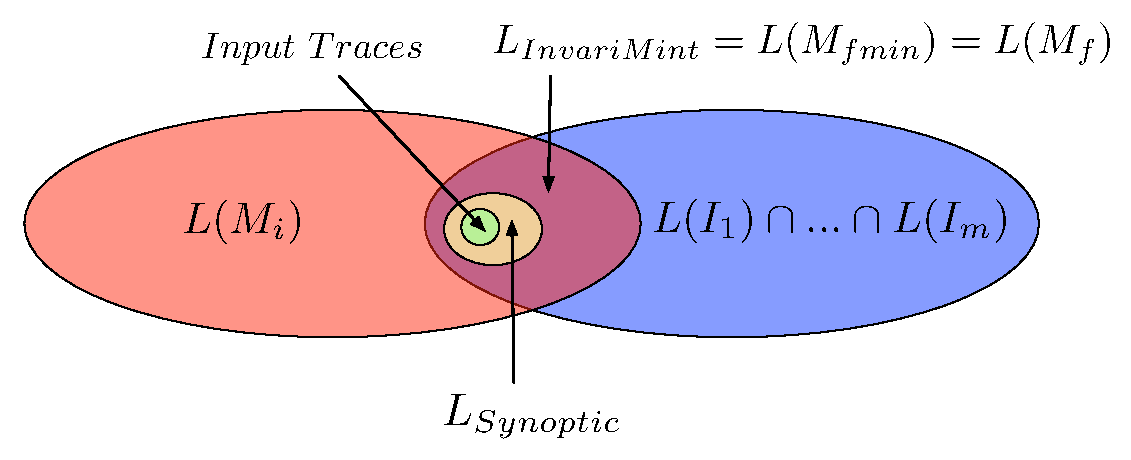
\includegraphics[width=0.95\columnwidth]{fig/language-venn.pdf}}
   \caption{This diagram illustrates the relationships between languages
    accepted by various models of the input traces. $L(M_i)$ is the language of
    the initial model which includes all of the input traces and is constrained
    only by the $NIFby$ invariants.
    $L(I_1) \cap \ldots \cap L(I_m)$ is the language of the intersected mined
    invariants. By design, $L(I_1)$ accepts all of the input traces.
    $L_{Synoptic}$ also accepts all of the input traces and is constrained by
    both the mined invariants and $M_i$. 
    Since Synoptic is non-deterministic, $L_{Synoptic}$ may vary given the same
    inputs but always respects the above constraints.
    $L_{InvariMint}$ is precisely the intersection of $L(M_i)$ and $L(I_1) \cap
    \ldots \cap L(I_m)$.
   } 
   \label{fig:language-venn}
\end{figure}


%%%%%%%%%%%%%%%%%%%%%%%%%%%%%%%%%%%%%%%%%%%%%%%%%%%%%%%%%%
\subsection{Constructing the final model}
%%%%%%%%%%%%%%%%%%%%%%%%%%%%%%%%%%%%%%%%%%%%%%%%%%%%%%%%%%
Define the DFA $M_f$ as the intersection $M_i \cap I_1 \cap \ldots
\cap I_m$ where $M_i$ is the initial model and $I_1, \ldots, I_m$
correspond to the set of mined
invariants defined in Section~\ref{sec:synoptic}.
By using the same invariants as Synoptic, we can both quantitatively and qualitatively
evaluate differences between models produced by the two techniques.

The corresponding language
$L(M_f)$ consists of all traces that
satisfy all of the mined and immediate invariants.  This language is generative
--- it includes $T$, the input traces, as well as all possible
stitchings of traces that satisfy the invariants. These stitchings are
possible traces allowed by the invariants but not yet observed in any input log.
Such traces are called synthetic traces, and exist in both Synoptic and
InvariMint models. These traces predict likely
future system behavior.

Having formed $M_f$ we can apply Hopcroft's classic DFA minimization
algorithm to $M_f$ to derive
$M_{f min}$. This algorithm guarantees that $M_{f min}$ is the smallest possible
DFA that accepts the same language as $M_f$. Figure~\ref{fig:language-venn}
summarizes the above discussion, which captures the
relationships between the languages accepted by $M_{f min}$,
$M_f$, and the other DFAs.

%%%%%%%%%%%%%%%%%%%%%%%%%%%%%%%%%%%%%%%%%%%%%%%%%%%%%%%%%%
\subsection{Implementation}
\label{sec:implementation}
%%%%%%%%%%%%%%%%%%%%%%%%%%%%%%%%%%%%%%%%%%%%%%%%%%%%%%%%%%

InvariMint uses the same parsing and invariant mining code used by Synoptic as
well as additional mining code to extract the immediate invariants.

The state machines manipulated by InvariMint are implemented as a layer above
the dk brics automata library~\cite{automaton}. This library provides regular expression parsing for
converting invariants to DFAs, as well as intersection and minimization
implementations of the algorithms described in Section~\ref{sec:Definitions}.
Our implementation provides an abstraction between the unicode alphabet
used by dk brics and the EventTypes mined from the input logs.

%%%%%%%%%%%%%%%%%%%%%%%%%%%%%%%%%%%%%%%%%%%%%%%%%%%%%%%%%%
\section{Evaluation}
\label{sec:evaluation}
%%%%%%%%%%%%%%%%%%%%%%%%%%%%%%%%%%%%%%%%%%%%%%%%%%%%%%%%%%
In practice, InvariMint not only infers useful summary models of the system
responsible for the input logs, but does so while addressing each of the
Synoptic limitations described in Section~\ref{sec:motivation}.

To evaluate the success of the formal languages approach, we also measure 
the relative efficiency of the two tools and compare
the final models generated by InvariMint with those generated by Synoptic.
% Discuss why walking the input traces didn't resolve the issue (Synoptic NFA to
% DFA translation)

%While implementing DFA
%minimization, for example, we realized an important distinction
%between invariants that are true for every trace (such as x Never Followed by y)
%and invariants that are only true globally (such as x Can be Followed by y).

%%%%%%%%%%%%%%%%%%%%%%%%%%%%%%%%%%%%%%%%%%%%%%%%%%%%%%%%%%
\subsection{Addressing Synoptic limitations}
%%%%%%%%%%%%%%%%%%%%%%%%%%%%%%%%%%%%%%%%%%%%%%%%%%%%%%%%%%

First, it is easy to add new types of invariants to InvariMint
as long as the invariants can be expressed as DFAs. This is how we recreated
Synoptic's initial model. This feature can also be used to more closely model
known features of systems. As one
example, consider some program in which an event $x$ must occur exactly twice before
some other event $y$. This would be a trivial addition to InvariMint, requiring
only some additional mining code and a regular expression for translating that
temporal relationship to a DFA. The same would be time
consuming to implement in Synoptic.

Second, InvariMint is much simpler to explain than Synoptic.
Whereas Synoptic uses highly specialized algorithms, DFA intersection and
minimization are both common, widely understood techniques for manipulating
state machines.

Third, InvariMint deterministically generates a globally minimal model that
satisfies all mined invariants. In contrast to Synoptic's refinement phase, the
order in which InvariMint intersects invariants has no affect on the final
model.

Finally, by referencing the input logs only once to mine invariants rather than continually
while constructing the final model, InvariMint scales better than
Synoptic on large logs.

%%%%%%%%%%%%%%%%%%%%%%%%%%%%%%%%%%%%%%%%%%%%%%%%%%%%%%%%%%
\subsection{Performance}
%%%%%%%%%%%%%%%%%%%%%%%%%%%%%%%%%%%%%%%%%%%%%%%%%%%%%%%%%%
InvariMint offers better scalability than Synoptic with respect to the size of
the input log because the algorithm avoids repeated references to the log while
inferring the final model. We measured scalability with respect to the size
of the input log by timing both Synoptic and InvariMint on logs of varying
size from the Reverse Traceroute system~\cite{ReverseTraceroute} which
determines return paths for packets on the Internet.
Figure~\ref{fig:performanceLogLine} plots the run time in milliseconds of both Synoptic and
InvariMint
on input logs ranging from 250 to 64,000 lines. 
Recorded times are the average of 10 executions measured after 10 warm-up
runs. 

As the size of the log increases, InvariMint is far more
efficient than Synoptic. Eventually parsing the input log and mining invariants dominates InvariMint's run
time as opposed
to the time taken to infer the final model.

These experiments only confirm that InvariMint is efficient with respect to the
size of the input log. In the future we hope to measure InvariMint's scalability
with respect to the number of log invariants. For all of the Reverse Traceroute logs,
the number of invariants (both mined and implicit) is lower than 200.

\begin{figure}
  \center
  {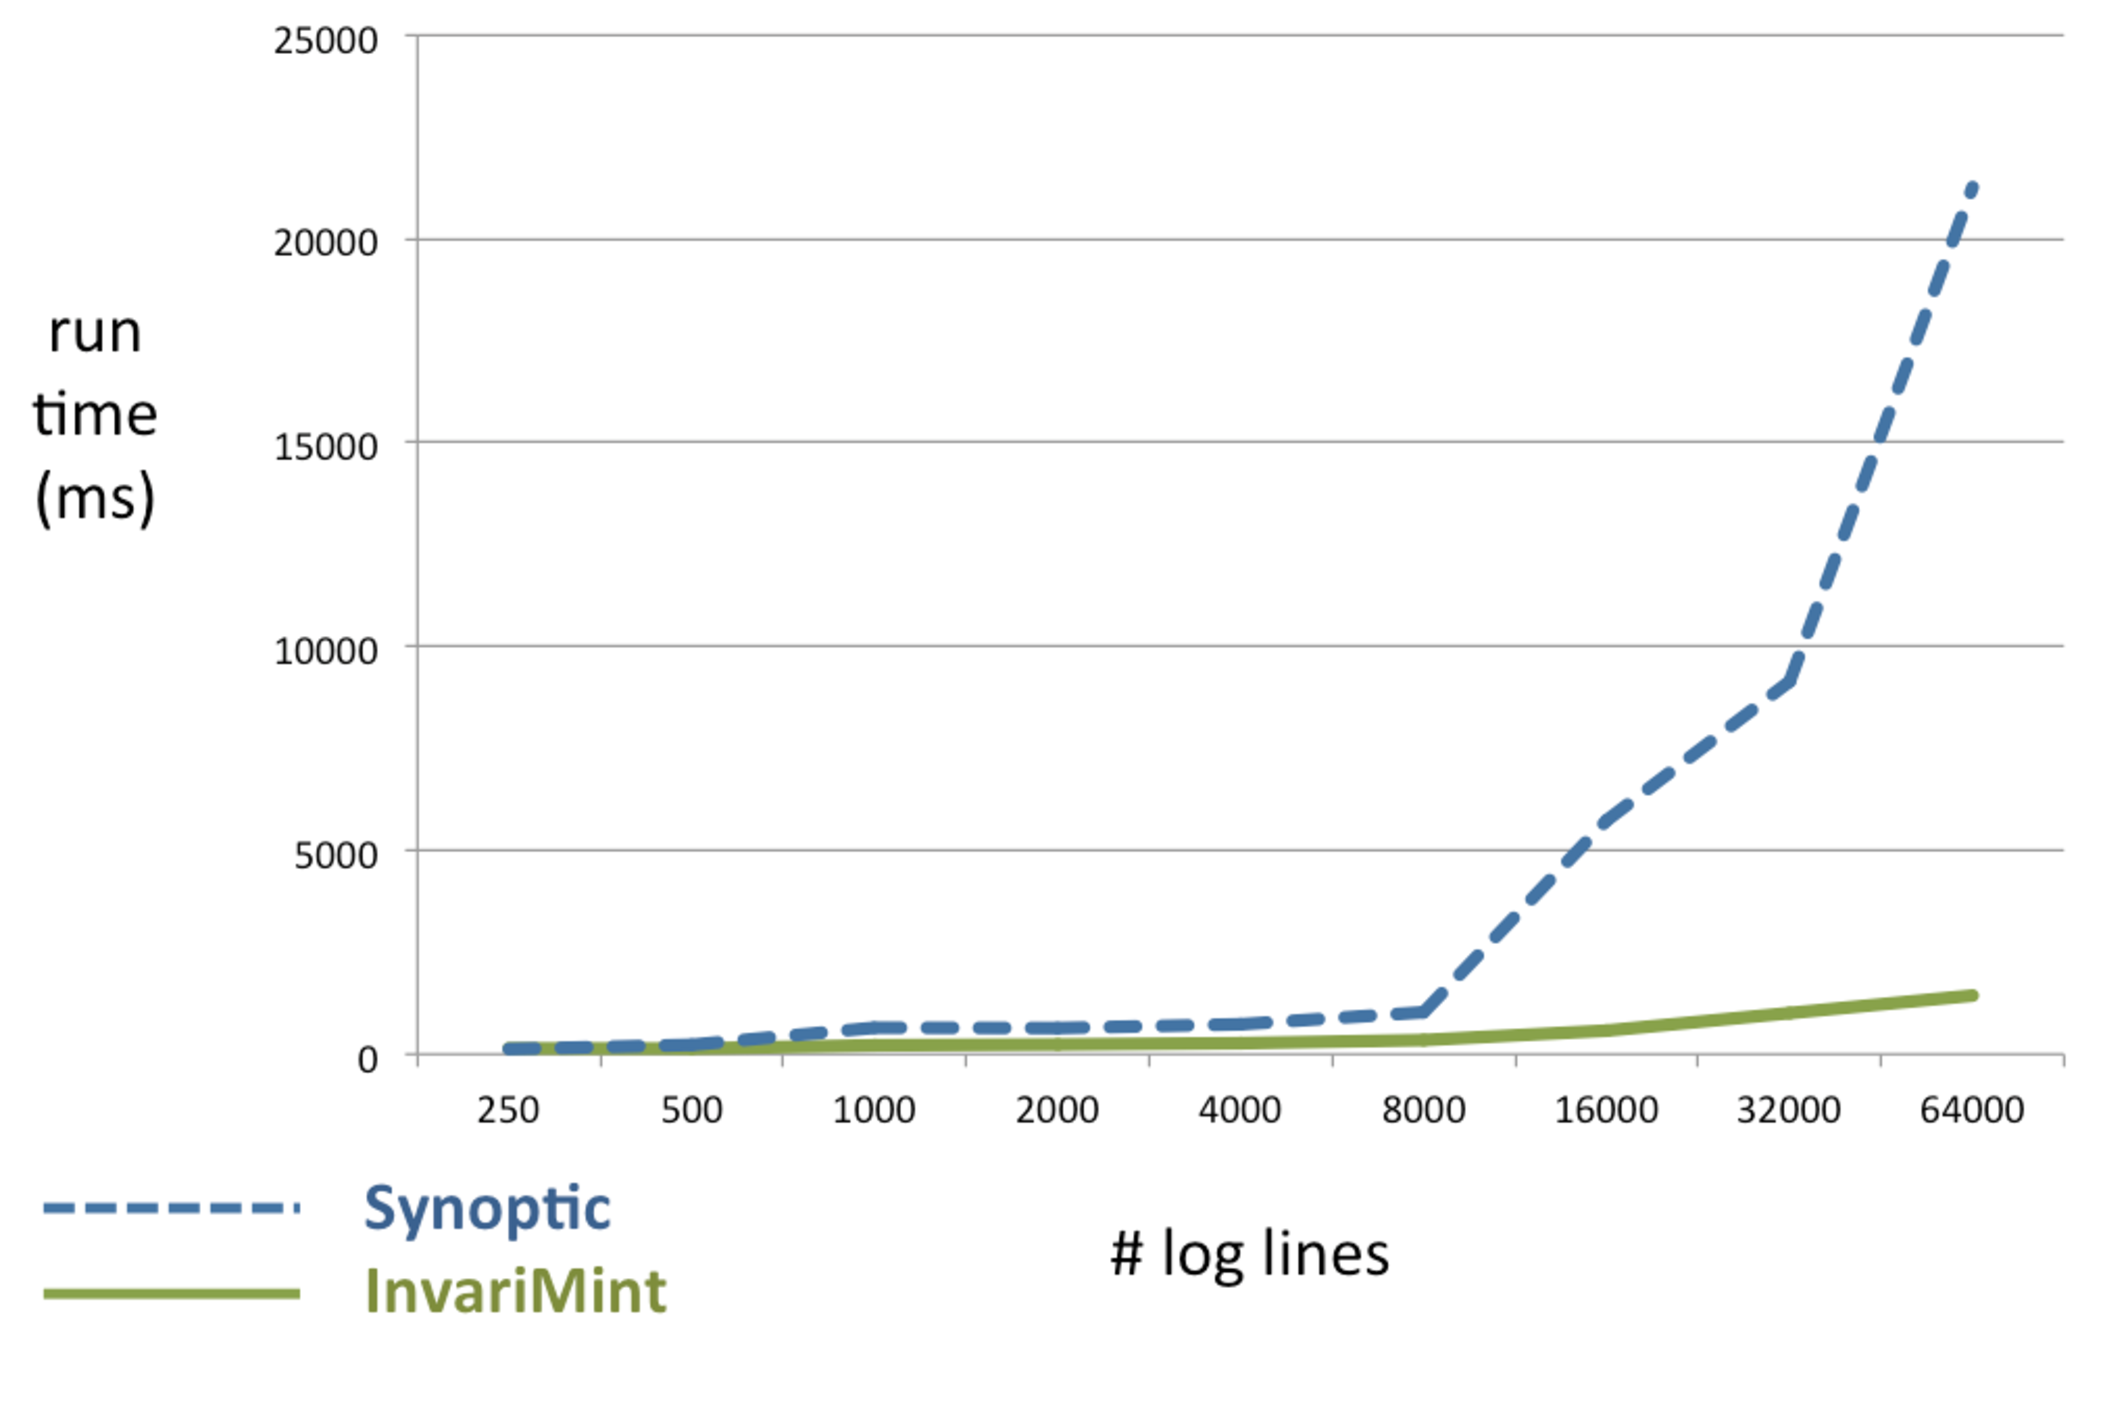
\includegraphics[width=\columnwidth]{fig/performanceLogLines.pdf}}
  \caption{Run time of Synoptic versus InvariMint as the size of the input log
  increased.}
  \label{fig:performanceLogLine}
\end{figure}

%%%%%%%%%%%%%%%%%%%%%%%%%%%%%%%%%%%%%%%%%%%%%%%%%%%%%%%%%%
\subsection{Model comparisons}
%%%%%%%%%%%%%%%%%%%%%%%%%%%%%%%%%%%%%%%%%%%%%%%%%%%%%%%%%%
Despite satisfying the same invariants and accepting all of the input traces,
InvariMint and Synoptic do not generate identical models. Exploring these
differences is useful for thinking about discrepancies between the techniques
and is important because the differences may make it harder or easier for
developers to use the models.

\begin{figure*}[t]
  \center
  {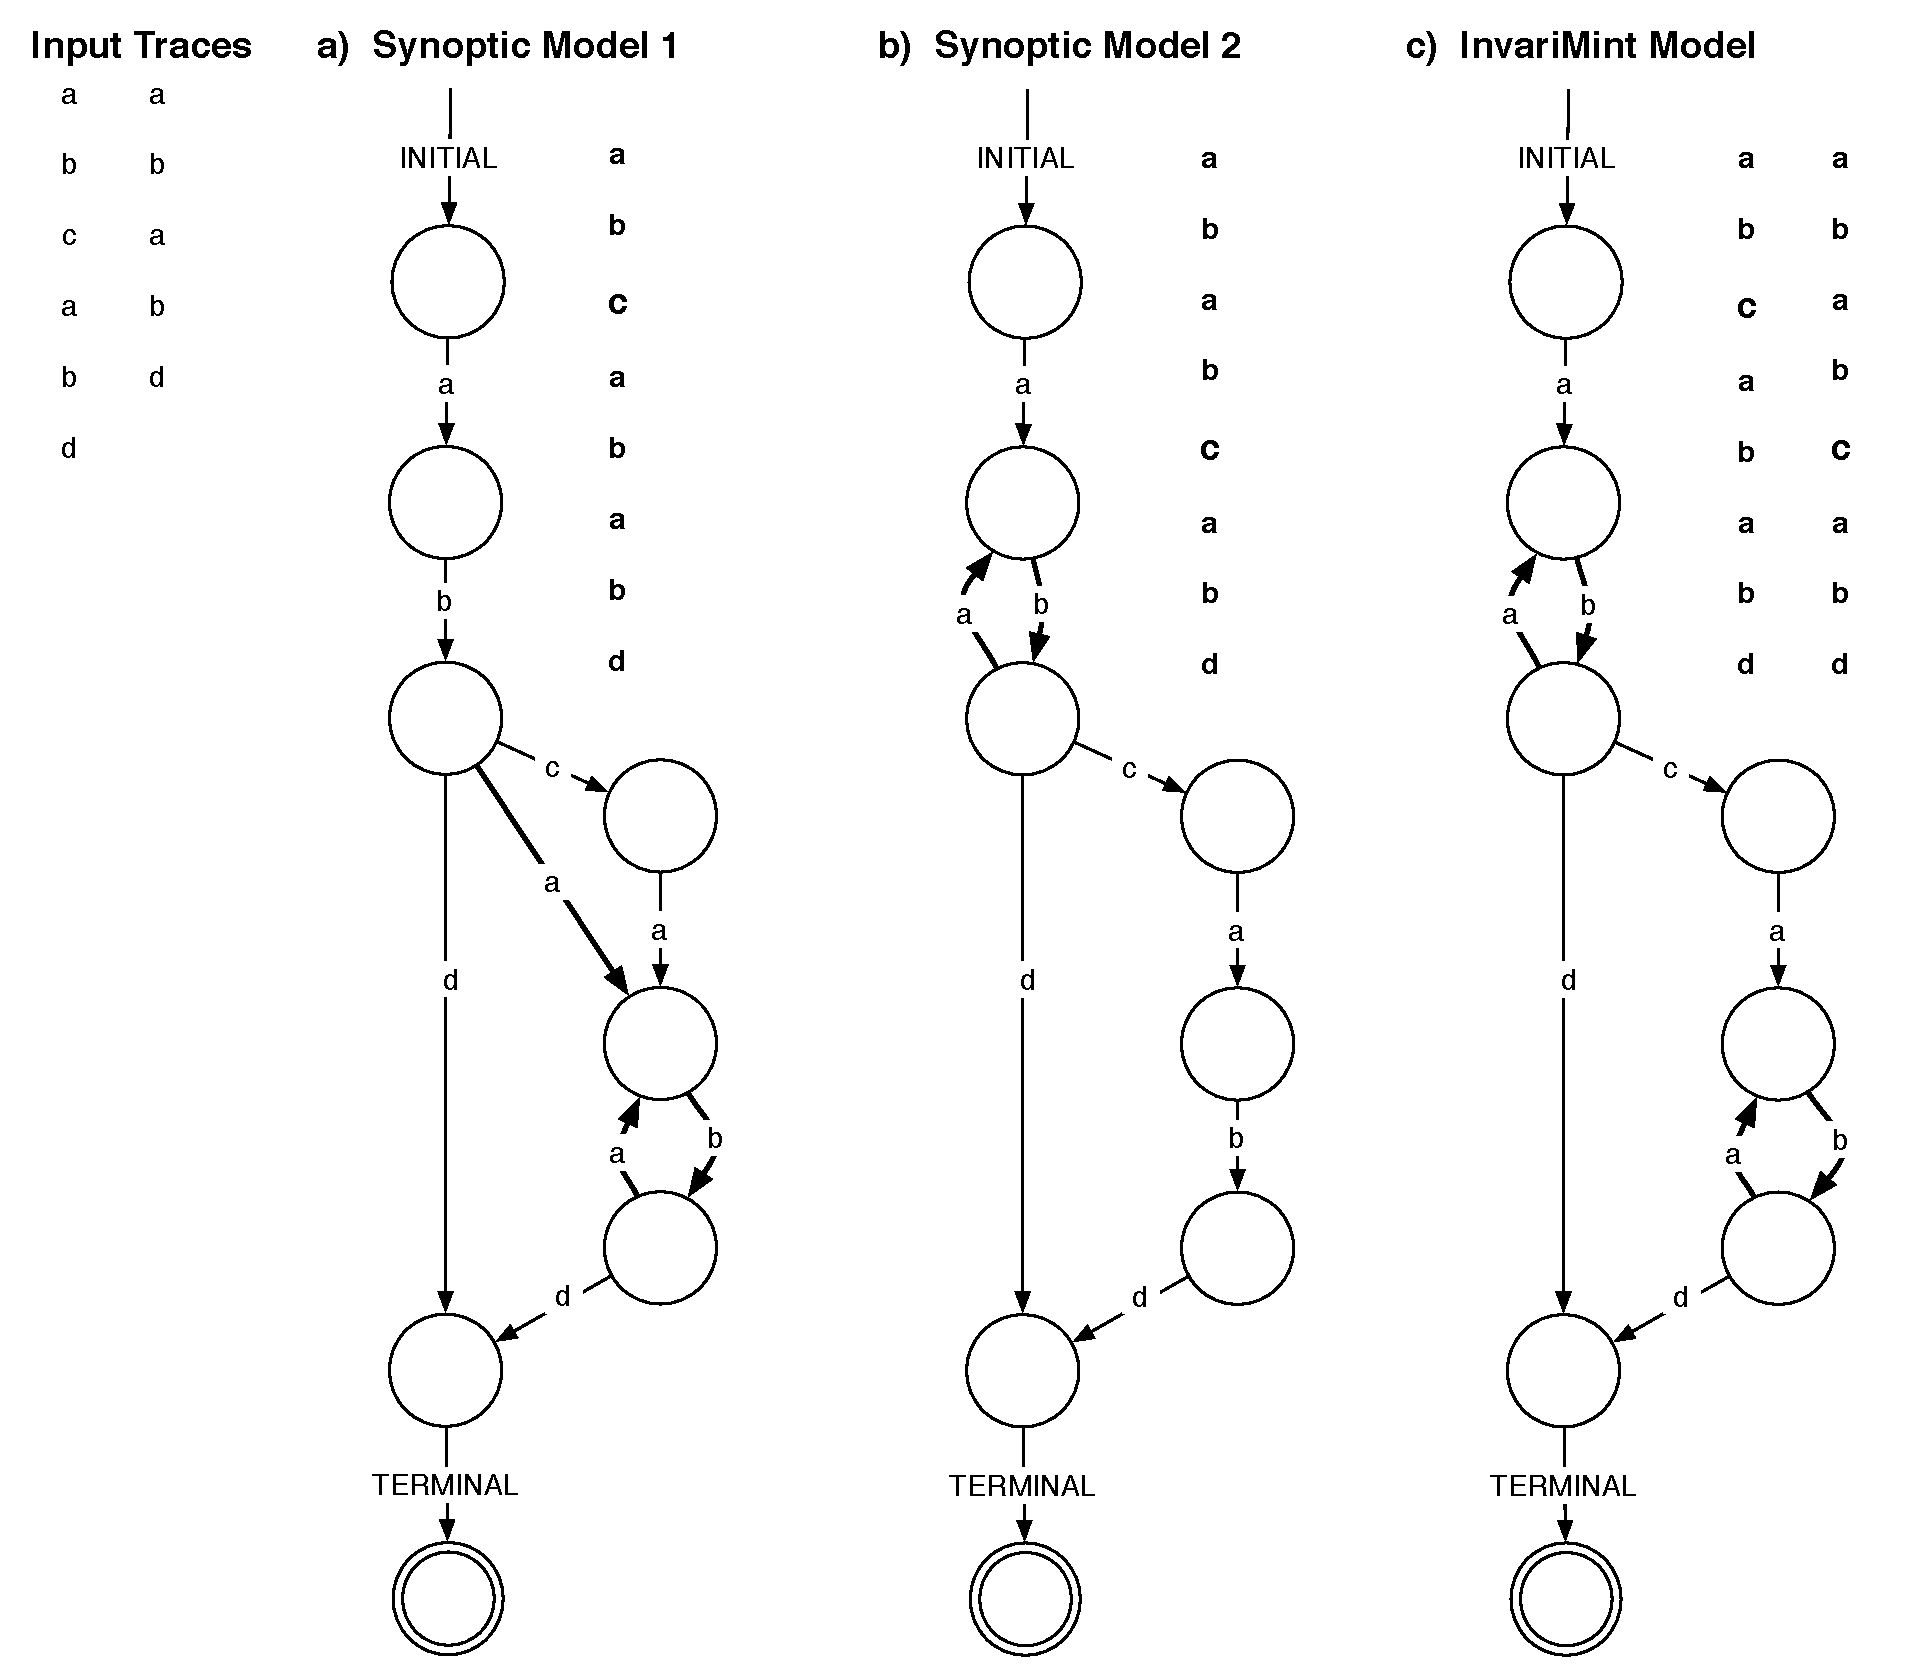
\includegraphics[width=\linewidth]{fig/union.pdf}}
  \caption{Models a and b are possible final Synoptic models given the provided input
  traces. Next to each model is an example of a synthetic trace accepted by that
  model but not the other. The corresponding InvariMint model, c, accepts the union
  of synthetic traces accepted by both Synoptic models.} 
  \label{fig:synthetic}
\end{figure*}

%%%%%%%%%%%%%%%%%%%%%%%%%%%%%%%%%%%%%%%%%%%%%%%%%%%%%%%%%%
\subsubsection{Union of Synoptic models}
%%%%%%%%%%%%%%%%%%%%%%%%%%%%%%%%%%%%%%%%%%%%%%%%%%%%%%%%%%
Synoptic generates a final model that accepts all of the input traces as well as
some synthetic traces satisfying all of the mined and immediate invariants.
Because Synoptic is non-deterministic, the set of synthetic traces accepted by
the final model may vary depending on the order in which invariants were
satisfied during refinement. Figure~\ref{fig:synthetic} illustrates an example
of this: there are two possible final Synoptic models satisfying
all log invariants for the given input traces, and these models accept a different set of synthetic traces.

This can be problematic for users. Consider the developer who finds a bug in
their system by examining a Synoptic model. After modifying their system, the
developer provides new input logs to Synoptic to verify that the bug is fixed.
Though the buggy behavior is gone, it is possible that some unrelated part of
the model has changed, leaving the developer to wonder whether they
unintentionally introduced additional modifications to the system.

InvariMint solves this issue by generating models deterministically.
Though not formally verified, we hypothesize that the final InvariMint model 
accepts the union of all possible synthetic traces accepted by any of
the corresponding Synoptic models. This is the case for the InvariMint
model in 
Figure~\ref{fig:synthetic} which accepts both sets of synthetic traces generated by different
Synoptic models.


Figure~\ref{fig:language-venn}
provides a visual illustration for the intuition behind this idea: the language accepted by InvariMint
is precisely the intersection of the initial model and each of the mined
invariants. Synoptic accepts a language that is some subset of that
intersection.

The union property is poised to have a number of benefits. First, it provides a bound for the set of
possible final Synoptic models which was previously an ambiguous space. Second,
the additional synthetic traces may be useful for users attempting
to predict the range of possible system behaviors for purposes such as generating
additional test cases. In future work we hope to conduct a
usability study to evaluate the utility of additional
synthetic traces. 

%%%%%%%%%%%%%%%%%%%%%%%%%%%%%%%%%%%%%%%%%%%%%%%%%%%%%%%%%%
\subsubsection{Spurious Edges}
%%%%%%%%%%%%%%%%%%%%%%%%%%%%%%%%%%%%%%%%%%%%%%%%%%%%%%%%%%
Assuming that the languages accepted by Synoptic models are always a subset of
the language accepted by a corresponding InvariMint model, the next question
is whether 
there are any traces accepted by an InvariMint model that are not
accepted by \emph{any} corresponding Synoptic model.

In fact, InvariMint models can accept synthetic traces that do not exist in any
corresponding Synoptic model. These are caused by \textbf{spurious edges} and
highlight an important distinction between the two techniques: underlying the Synoptic models
are specific event instances, whereas
InvariMint deals only with event types.

During refinement and coarsening, 
Synoptic maintains partitions containing one or more
concrete instances of that partition's event type from some input trace.
For each event instance $a$ in the partition, there exists an incoming edge from some
partition containing the event instance that immediately preceded that instance $a$ and there
exists an outgoing edge that leads to some partition containing
the event instance that immediately followed $a$.
Synoptic models thus have the property that every edge in the final model corresponds
to two successive events in at least one input trace. In other words, every edge
respects the \emph{edge-coverage property}.

The Synoptic model accepts some synthetic traces -- traces not contained within
the set of 
input traces -- but these are limited by the edge-coverage property.

InvariMint models in contrast have no notion of input traces and are concerned
only with the temporal relationships between event types.
Because InvariMint models
do not have the edge-coverage property, they are
more permissive than Synoptic models, accepting a wider range of synthetic
traces.

Figure~\ref{fig:spurious} illustrates an example of this.
The Synoptic model allows only the set of input traces in its final model.
The InvariMint model allows 
an additional $INITIAL-x-a-y-TERMINAL$ synthetic trace because no mined
invariant prohibit it.

\begin{figure}[t!]
   \center
   {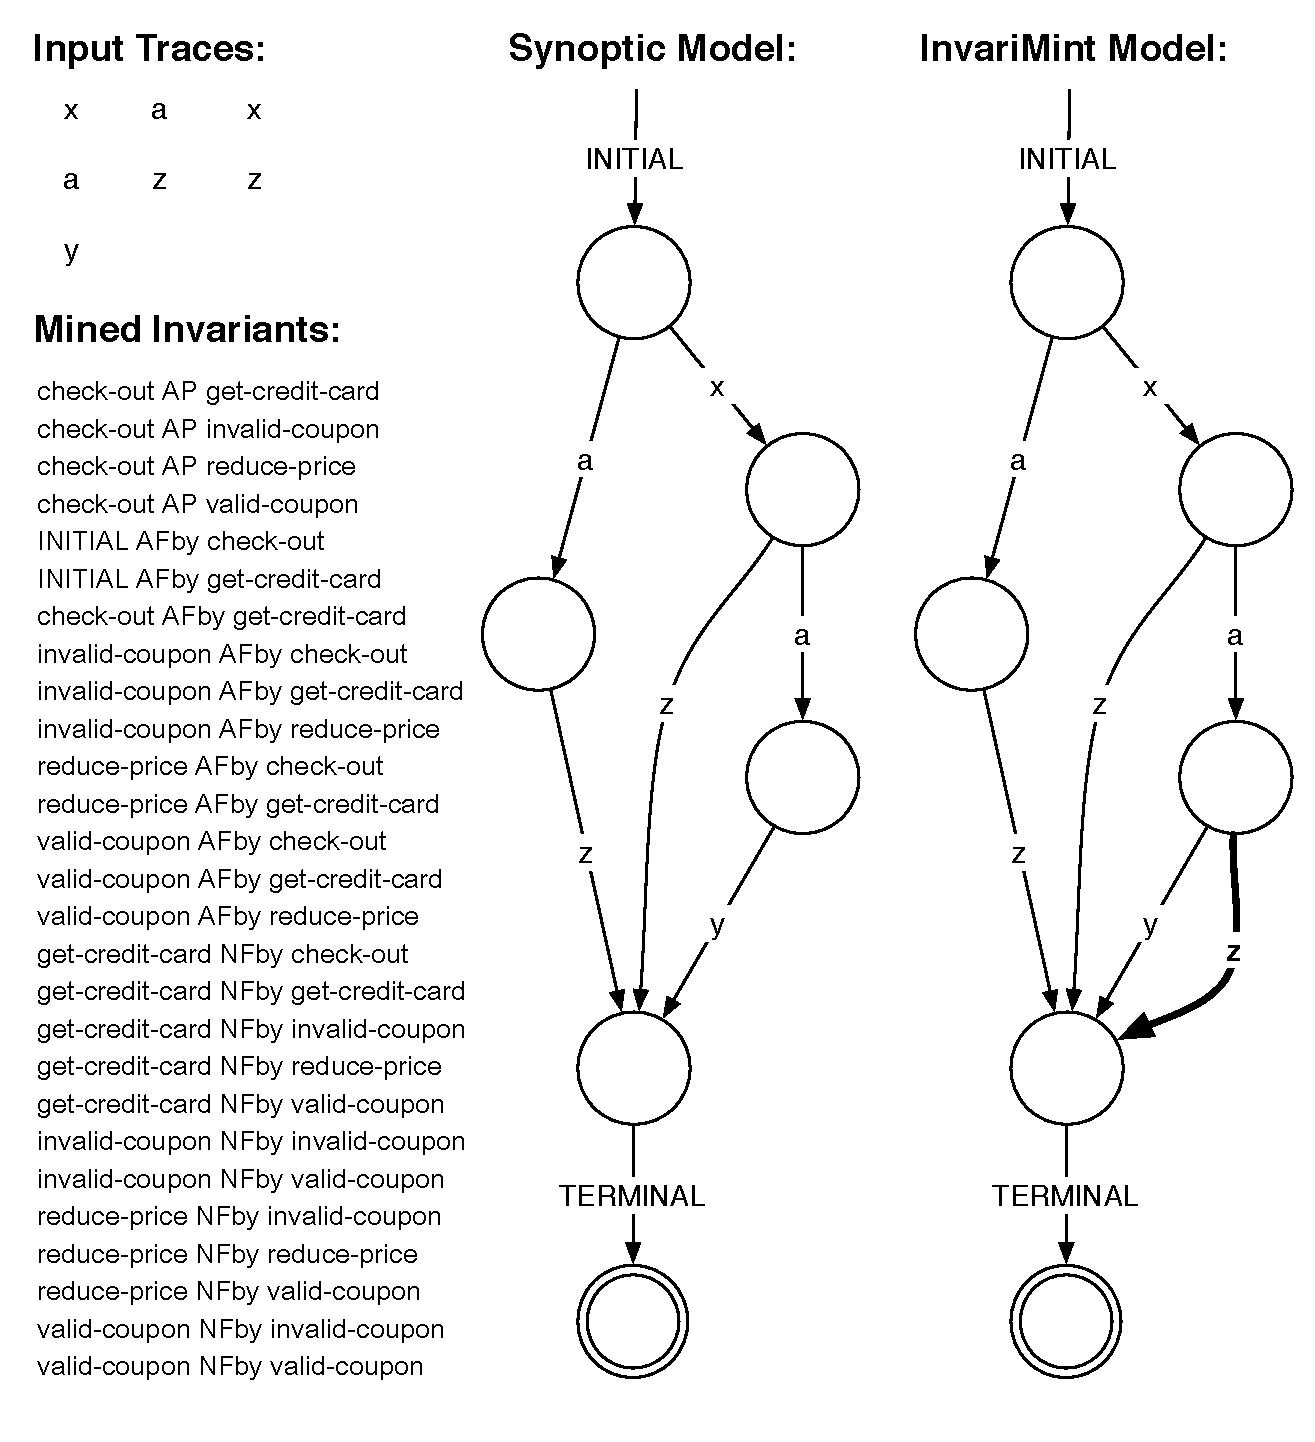
\includegraphics[width=0.95\columnwidth]{fig/spurious.pdf}}
   \smallskip
   \caption{An abstract example of a spurious edge in an InvariMint model. The input traces
   and mined invariants are shown at left. Each edge in the Synoptic model
   (translated to an InvariMint-style DFA for easier comparison)
   corresponds directly to an event in some input trace. The InvariMint
   model is almost identical to the Synoptic model but includes an additional 
   $z$ edge from $a$ to $TERMINAL$. This transition does not map to any event in the
   input logs so violates the edge-coverage property and is spurious.
   This spurious $z$ edge is allowed by InvariMint because elsewhere an event
   $z$
   immediately followed an event $a$ and none of the other invariants restrict this
   particular instance of $z$.}
   \label{fig:spurious}
\end{figure}

More concretely, because an event $z$ immediately followed an event
$a$ in at least one input trace, the $a~NIFby~z$ invariant was not mined during
construction of 
the initial model and every instance of an event $a$ in the InvariMint model can be
immediately followed by an event $z$ unless prohibited by 
some other invariant. The left-most event $a$ in the InvariMint model in Figure~\ref{fig:spurious},
for example, is not followed by an event $y$ even though $y$ can immediately
follow $a$ because that would allow traces violating the 
$x~AP~y$ invariant.

The $z$ edge in the InvariMint synthetic trace would map to an $a$--$z$
edge in the corresponding state-based model used by Synoptic. There does not
exist any input trace that would traverse the $z$ edge in this model, and thus
the edge is an 
example of a spurious edge.

%%%%%%%%%%%%%%%%%%%%%%%%%%%%%%%%%%%%%%%
\subsubsection{Removing spurious edges}
%%%%%%%%%%%%%%%%%%%%%%%%%%%%%%%%%%%%%%%
To best approximate Synoptic, InvariMint models should not contain any spurious
edges. However, we have not yet developed an adequate way to remove these 
edges from InvariMint models.

One plausible way to remove spurious edges is to traverse the input traces
during one additional post-processing step and remove any edges in the final
InvariMint model violating the edge-coverage property.

A problem with this
strategy is that Synoptic generates NFAs with the edge-coverage property whereas
InvariMint generates DFAs. Translating Synoptic models to DFAs generates models
that accept the same language as the original model but creates a model that may
violate the edge-coverage
property.

This is due to additional edges and states introduced by the NFA-to-DFA
translation. Thus InvariMint models can contain
edges
that both violate the edge-coverage property and are spurious, but 
can also contain edges that 
violate the edge coverage property but if removed would restrict
the language of the model in ways that the corresponding Synoptic model does not.

For example, applying the post-processing operation to remove spurious edges
on the InvariMint model in Figure~\ref{fig:synthetic} would remove the edges
that allow the a-b-c-a-b-a-b-d synthetic trace. The resulting language 
would no longer be the union of languages accepted by all Synoptic models.

Spurious edges reveal a loss of context in InvariMint models. Synoptic models
are more nuanced, preserving greater trace-specific information.
Given a Synoptic model, it is possible to query specific edges
to reveal precisely which 
input traces allowed that transition between events. This can be useful, for
example, to pinpoint
the precise executions in which a bug appeared. The mined invariants used by
InvariMint do not capture any trace specific information.

Less context-sensitivity is not necessarily a bad thing: the InvariMint models
are more
general and ignore individual trace idiosyncrasies, leading to smaller
models as more states can be merged. As the scale of the input grows, 
model brevity and efficiency may prove to be more valuable than trace-specific
information.

%%%%%%%%%%%%%%%%%%%%%%%%%%%%%%%%%%%%%%%%%%%%%%%%%%%%%%%%%%
\section{Generalizing the Technique}
\label{sec:generalizing}
%%%%%%%%%%%%%%%%%%%%%%%%%%%%%%%%%%%%%%%%%%%%%%%%%%%%%%%%%%
Synoptic is only one of the many algorithms used to infer models from
executions.  These techniques are difficult to compare and nearly impossible
to combine.  Some are slow, and some produce models that may not
be minimal. 

One of the advantages of the InvariMint approach is that it
provides a way to compare and combine different model inference approaches on the
same terms, and does so in an efficient, deterministic way.
In this section, we will first describe kTails ~\cite{kTailsOrigin}, a widely
used algorithm for FSM inference. We will then illustrate how kTails can
be expressed by composing invariant DFAs. We argue that InvariMint offers a
unifying framework for model inference methods by characterizing the existing
techniques in terms of invariant DFAs.


%%%%%%%%%%%%%%%%%%%%%%%%%%%%%%%%%%%%%%%%%%%%%%%
\subsection{kTails}
%%%%%%%%%%%%%%%%%%%%%%%%%%%%%%%%%%%%%%%%%%%%%%%

kTails is a coarsening algorithm for inferring concise models.
The algorithm begins with a fine-grained representation of a model in
which each event instance (not event type) is mapped to its own partition as in
Figure~\ref{fig:ktails}a.

kTails then iteratively merges pairs of
k-equivalent partitions. These are partitions in the model that are roots of
identical sub-graphs 
up to depth k. The resulting graphs after applying $k = 0$ and $k = 1$ to the
model in Figure~\ref{fig:ktails}a are shown in ~\ref{fig:ktails}b and
~\ref{fig:ktails}c respectively. 

The initial kTails graph is analogous to a trace graph for Synoptic in which
each execution trace from the input logs is a single path from the INITIAL to
TERMINAL nodes. It is possible to infer Synoptic-style models by simply applying
kTails to a trace graph for arbitrary values of k. Synoptic's initial model, in
which all events of the same type are merged, is
equivalent to running kTails on the trace graph with $k = 0$.

%%%%%%%%%%%%%%%%%%%%%%%%%%%%%%%%%%%%%%%%%%%%%%%
\subsection{Representing kTails using InvariMint}
%%%%%%%%%%%%%%%%%%%%%%%%%%%%%%%%%%%%%%%%%%%%%%%


\begin{figure}
   \center
   {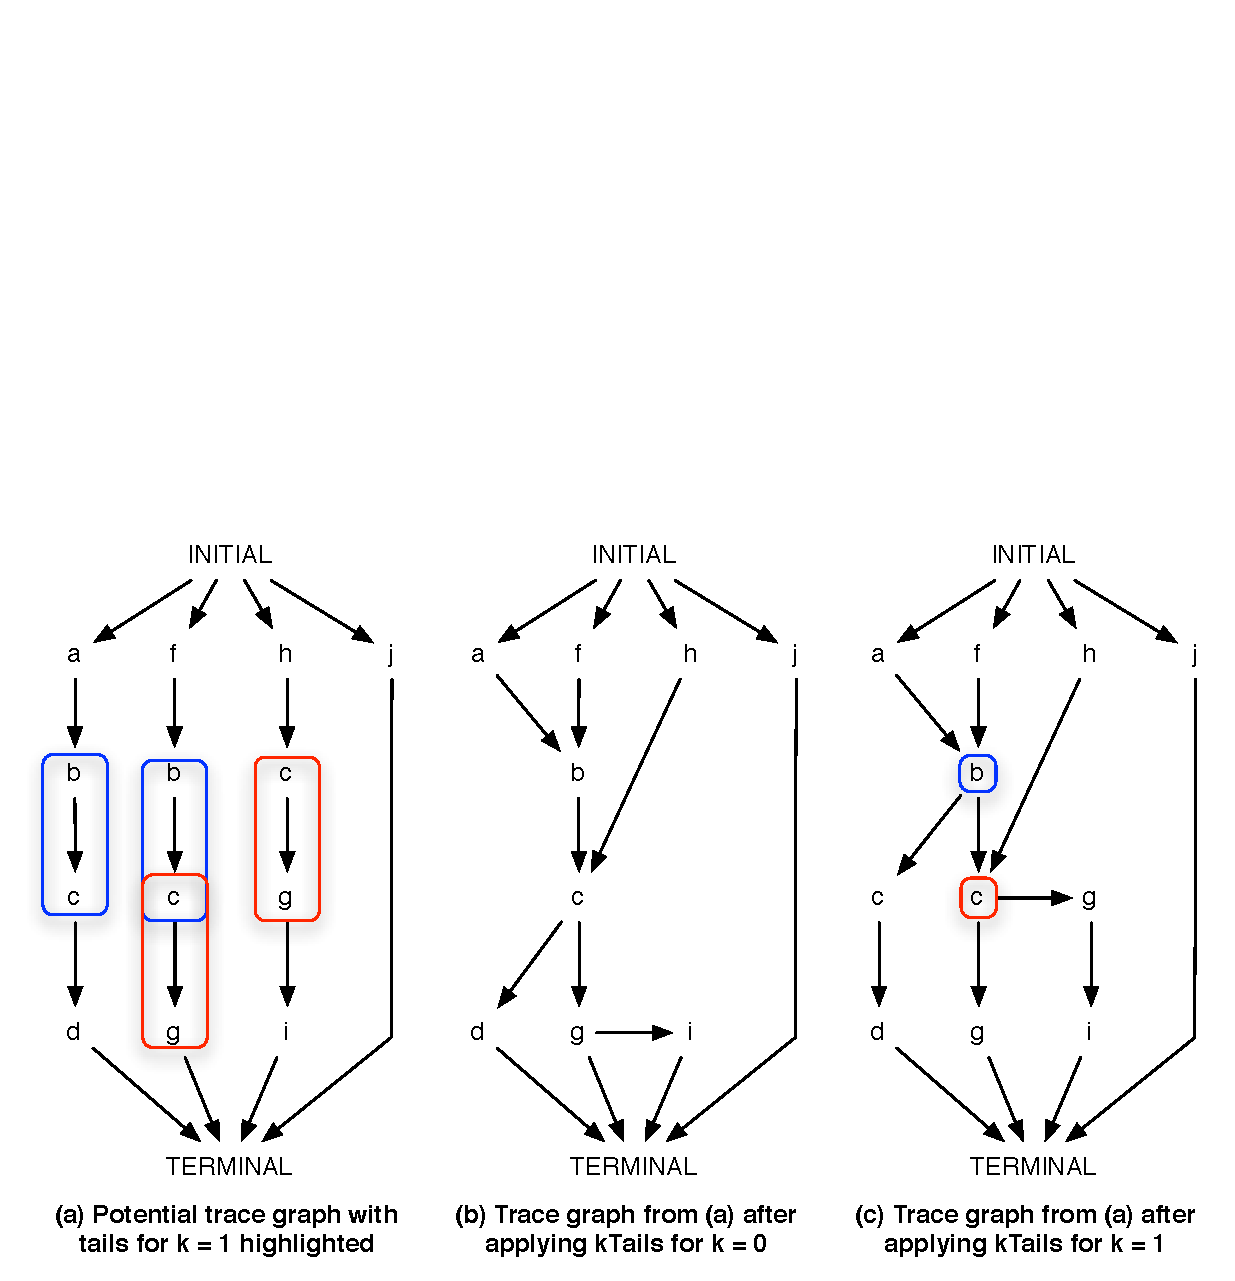
\includegraphics[width=0.95\columnwidth]{fig/ktails.pdf}}
   \caption{A sample trace graph and its corresponding models using
   InvariMint for kTails for k = 0 and k = 1.}
   \label{fig:ktails}
\end{figure}


\begin{figure}
   \center
   {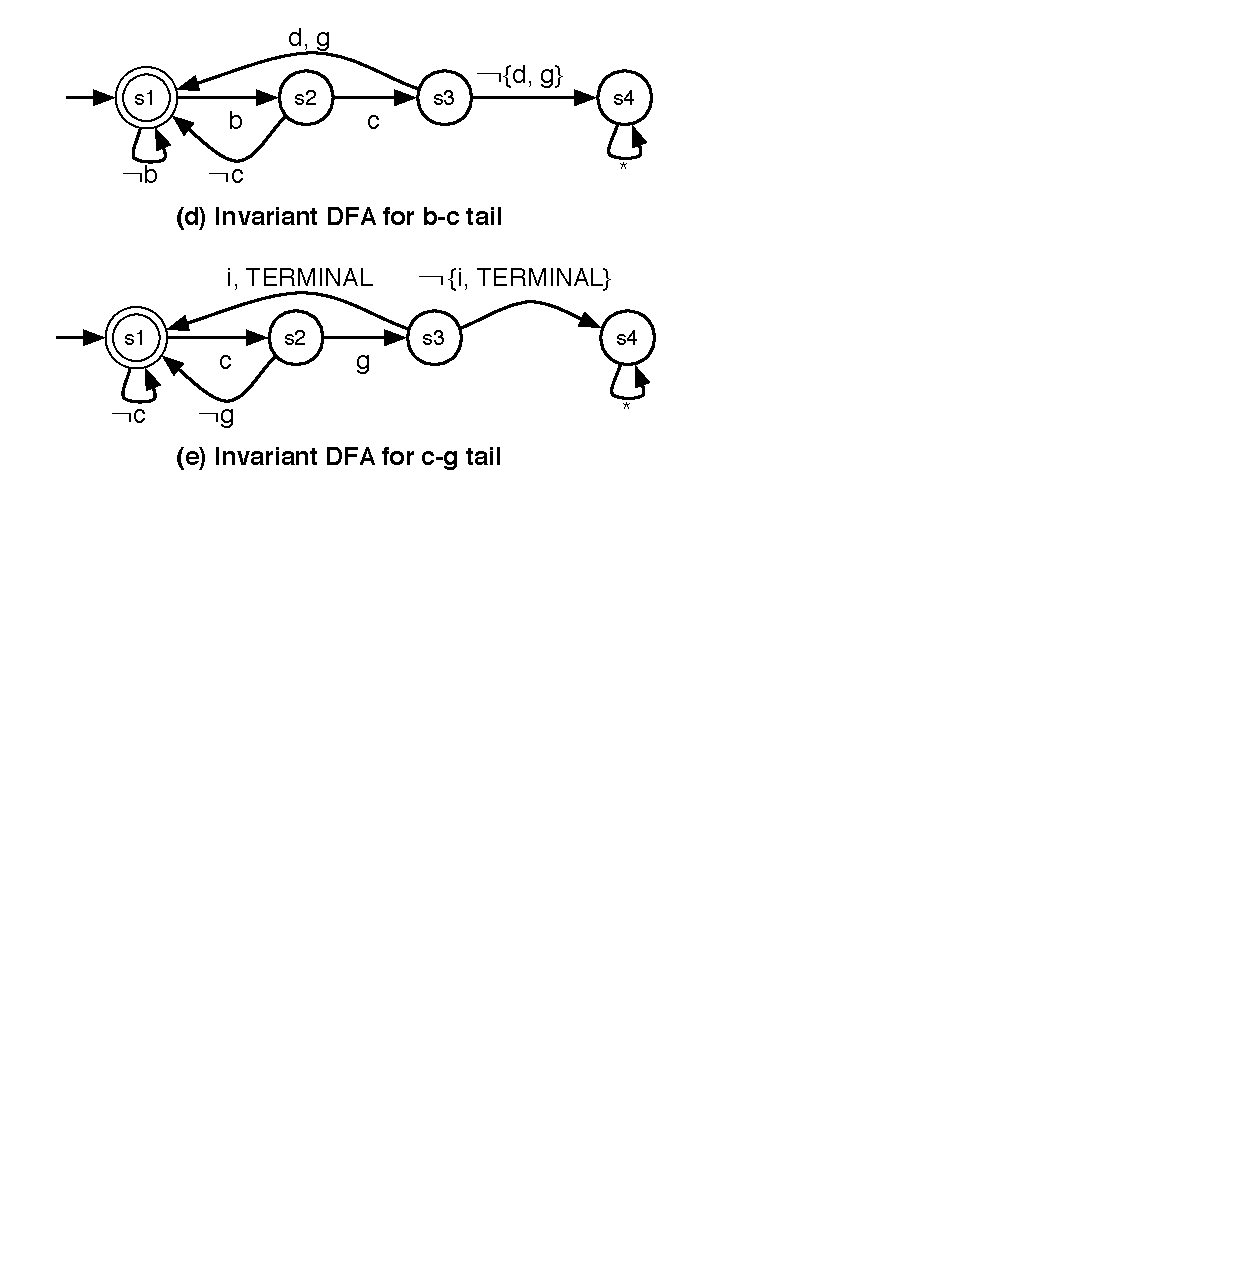
\includegraphics[width=0.95\columnwidth]{fig/tails.pdf}}
   \caption{Invariant DFAs for the tails in Figure~\ref{fig:ktails}a for
   $k = 1$.}
   \label{fig:tails}
\end{figure}


When k = 0, kTails merges all event instances of the same type which is
precisely equivalent to Synoptic's initial model and can be constructed with
InvariMint using the \emph{Never Immediately followed by} invariants. An example
of this is shown in Figure~\ref{fig:ktails}b.

For $k > 0$, invariants can describe tails of length k in
the model. To construct these, we mine all sub-graphs of depth $k + 1$ in the initial graph
that are shared by \textbf{at least two traces}. For all such tails, the set of
events that can immediately follow the tail are also recorded.
Each sub-graph is then translated into
an invariant DFA which stipulates that if a tail is seen, it must be immediately followed by
one of the next possible follow events. Figure~\ref{fig:tails} illustrates
these DFAs for $k = 1$.

Using these translation mechanisms, InvariMint is able to express the key properties
of kTails simply by taking the
intersection of all immediate invariants and each of the tail
invariants.

InvariMint offers a unifying framework for inferring models from executions by 
reducing other inference techniques to the set of invariants
that describe the essential properties of their models. Because these invariants
are all describable with formal languages,
it is possible to generalize, combine, and compare existing
techniques simply by adjusting the set of invariants used to construct the final
model.

For example, using InvariMint a developer would be able to merge k-tails of
varying length depending on the event type, and could intersect that model with
whichever temporal Synoptic invariants deemed most appropriate. This flexibility
provides a way for developers to better explore the space of formal
specification and to quickly create customized hybrid inference algorithms.

%%%%%%%%%%%%%%%%%%%%%%%%%%%%%%%%%%%%%%%%%%%%%%%%%%%%%%%%%%
\section{Conclusion}
\label{sec:conclusion}
%%%%%%%%%%%%%%%%%%%%%%%%%%%%%%%%%%%%%%%%%%%%%%%%%%%%%%%%%%

Synoptic is a tool for turning complex executions logs into convenient summary models
for analyzing systems. It infers these models by capturing key temporal
properties of the input logs. InvariMint
implements a new model inference engine for constructing similar models. The
InvariMint technique uses a formal languages perspective to express log
invariants which offers improvements over Synoptic's refinement and coarsening
algorithms:

(1) Turning logs into models offers an easy-to-create and easy-to-use
way to analyze systems. By using familiar DFA operations to infer these models,
the InvariMint process is easy for users to understand.

(2) InvariMint is more scalable than Synoptic. The InvariMint model inference technique
refers to the input traces once which makes the DFA intersection and minimization
operations more efficient than refinement and coarsening.

(3) Whereas Synoptic generates models non-deterministically, InvariMint is both
deterministic and captures all possible behaviors allowed by Synoptic models.

Additionally the formal language perspective is extensible: InvariMint makes it trivial to model
any system behavior that can be expressed as a finite state machine. This
generic approach allows InvariMint to be compatible with other inference
techniques, and we believe that it is a unifying framework for generalizing,
combining, and comparing those existing methods.


%%%%%%%%%%%%%%%%%%%%%%%%%%%%%%%%%%%%%%%%%%%%%%%%%%%%%%%%%%%%%%%%%%%%%%%%%%%%
% End Matter
%%%%%%%%%%%%%%%%%%%%%%%%%%%%%%%%%%%%%%%%%%%%%%%%%%%%%%%%%%%%%%%%%%%%%%%%%%%%

{
\bibliographystyle{acm}
\small
\bibliography{paper}
}

%\begin{appendices}
%\input{appendix}
%\end{appendices}

\end{document}

%%%%%%%%%%%%%%%%%%%%%%%%%%%%%%%%%%%%%%%%%%%%%%%%%%%%%%%%%%%%%%%%%%%%%%%%%%%% 
%%%%%%%%%%%%%%%%%%%%%%%%%%%%%%%%%%%%%%%%%%%%%%%%%%%%%%%%%%%%%%%%%%%%%%%%%%%%

